Nous avons ainsi étudié trois types d'échantillons différents :\\
\begin{itemize}
    \item Le brut, monocristallin, en sortie de fonderie
    \item L'alliage après remise en solution (premier traitement thermique)
    \item L'alliage en fin de traitement, après les deux revenus.\\
\end{itemize}


Nous devons donc étudier leur microstructure pour déterminer l'influence des 
différents traitements thermiques sur l'alliage, étant donné que cette microstructure
est le paramètre clé qui va déterminer les propriétés mécaniques de l'alliage,
et notamment sa résistance au fluage.

\subsection*{Echantillon brut de fonderie}

Étudions tout d'abord les propriétés du brut sortant de la fonderie.\\


\begin{figure}[H]
    \centering
    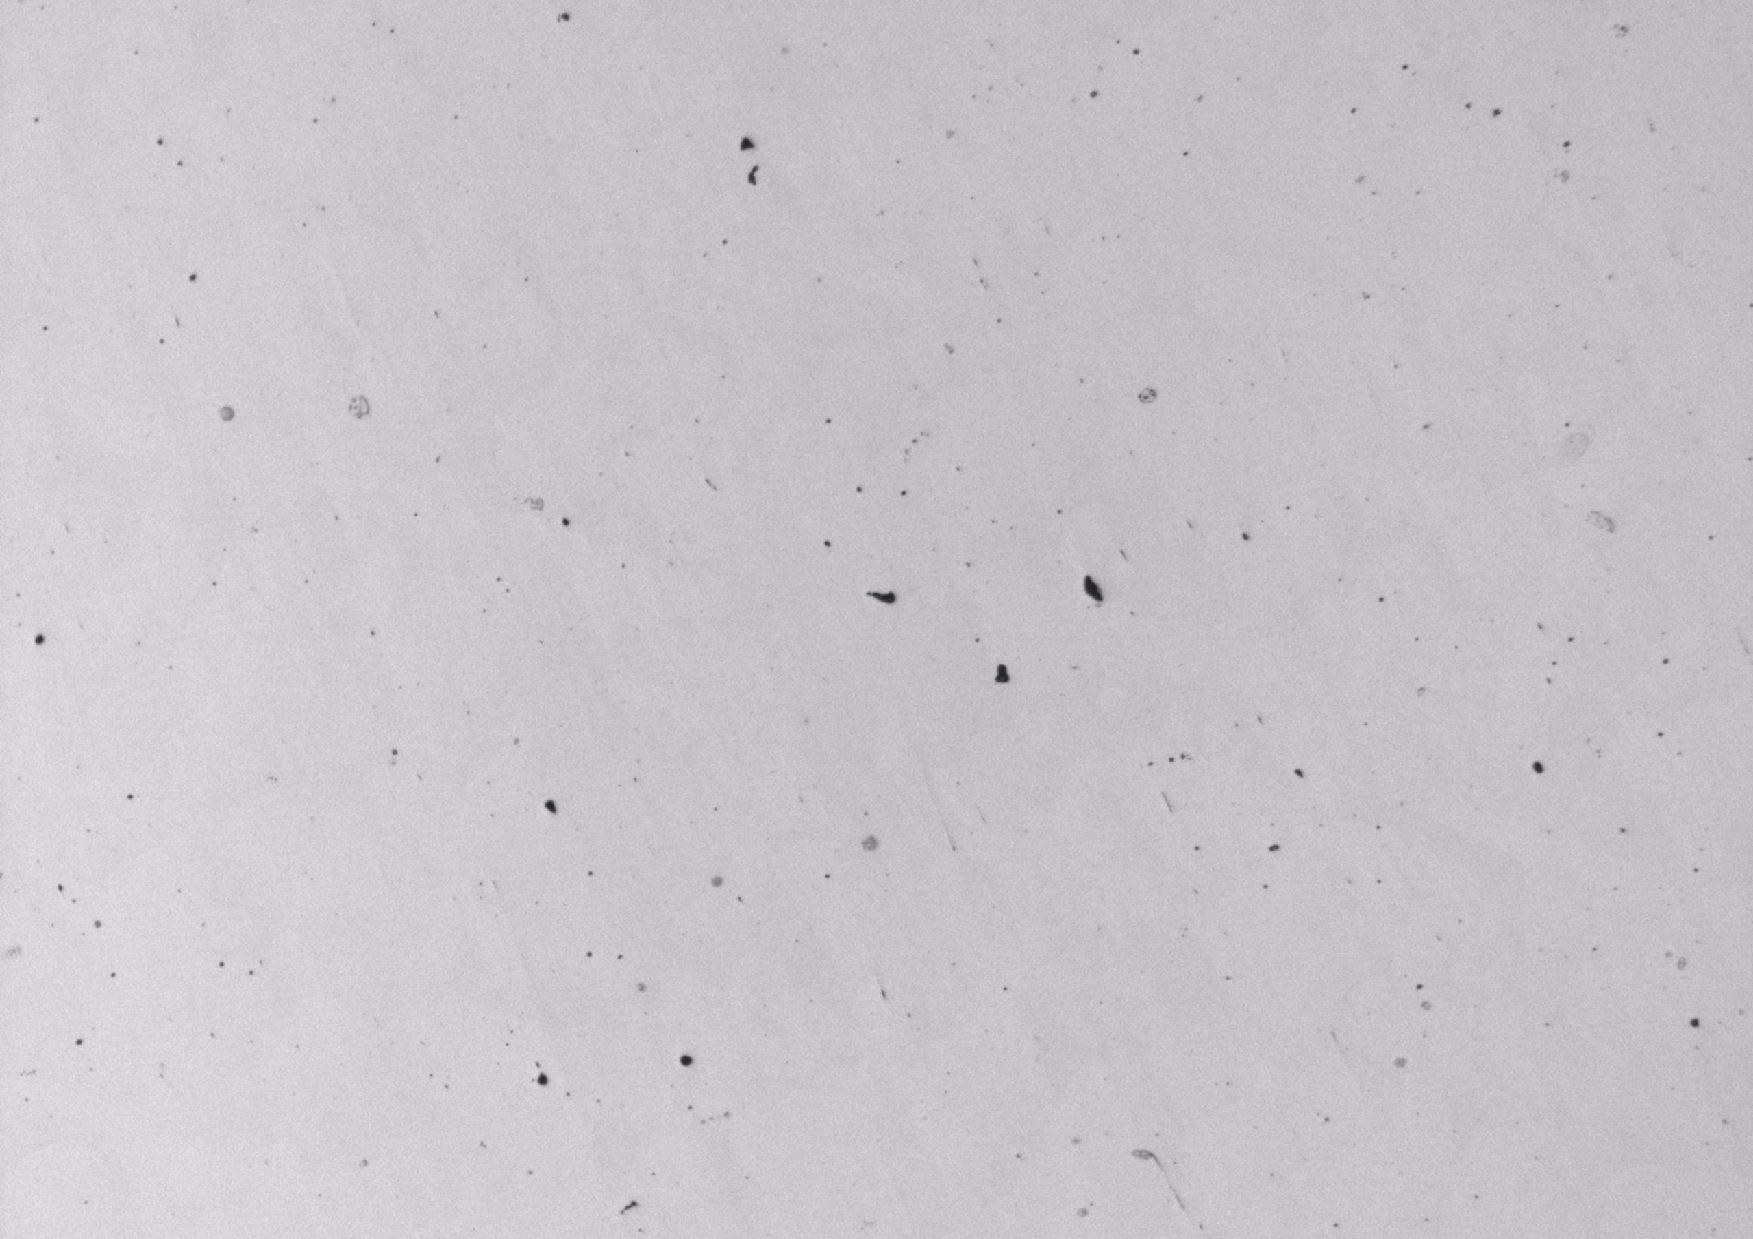
\includegraphics[width=0.75\textwidth]{images_optique/brut2.pdf}
    \caption{Echantillon brut de fonderie vu au microscope optique}
    \label{fig:brut_optique}
\end{figure}


Vu au microscope optique, sa surface (après polissage) est lisse
et présente peu de défauts. Cependant, la surface possède 
également de petites tâches noires : ces tâches sont des \emph{pores},
c'est à dire des trous à la surface de l'échantillon. Il y a à ces endroits 
des lacunes importantes dans la maille cristalline, et il manque donc 
une petite portion du matériau. Nous observons également de plus 
petites tâches grises : il s'agit d'agrégats eutectiques, formés 
lors du refroidissement du liquide.\\



On mesure la proportion de défauts visibles au microscope optique à l'aide du 
logiciel d'analyse d'images ImageJ. Nous obtenons les résultats suivants : \\


\begin{table}[H]
    \centering
    \caption{Proportion des différents défauts dans l'échantillon brut de fonderie}
    \begin{tabular}{|c|c|}
        \hline
        \textbf{Type de défaut}  & \textbf{Proportion observée}  \\
        \hline
        Pores               & $0,340$ \% \\
        Agrégats eutectiques & $0,252$ \% \\
        \hline
    \end{tabular}
    \\
    \label{tab:proportions_defauts_brut}
\end{table}


Nous voyons ainsi qu'il y a une quantité significative de défauts au sortir de la fonderie.\\


Les agrégats eutectiques apparaissent pendant le refroidissement 
et la solidification du liquide. En effet, la vitesse de refroidissement dans 
la pièce est très difficile à contrôler précisément, et est donc nécessairement
inhomogène. Ainsi, certaines zones vont commencer à solidifier avant d'autres, et 
vont donc modifier la composition chimique du liquide qui les entoure. 
Les dendrites, qui sont les parties qui solidifient en premier, sont composées 
principalement de phase $\gamma$ (d'après le diagramme de phases nickel-aluminium, 
figure \ref{fig:diagramme_phases_Ni_Al}), ce qui va modifier l'équilibre dans le liquide.
Les espaces inter-dendritiques vont ensuite se former,  plus riches en phase $\gamma'$, 
suivis enfin par les agrégats eutectiques composés de phase $\gamma'$.


\begin{figure}[H]
    \centering
    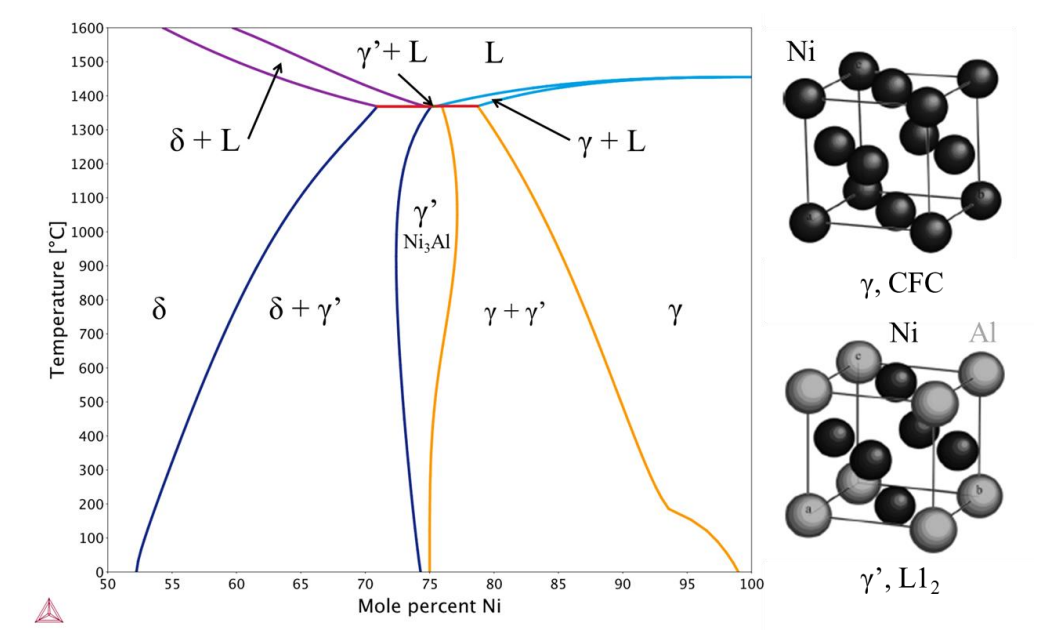
\includegraphics[width=0.75\textwidth]{images/diagramme_phase.png}
    \caption{Diagramme Ni-Al avec les structures cristallines des phases $\gamma$ et $\gamma'$}
    \label{fig:diagramme_phases_Ni_Al}
\end{figure}

% Quand on regarde le diagramme de phases nickel-aluminium, nous voyons que 
% lors de la solidification, le liquide va s'appauvrir en nickel et sa composition
% va tendre vers celle du liquide eutectique. Cela conduit donc à la formation de zones
% donc la composition est celle de l'assemblage $\gamma$/$\gamma'$, et d'autres zones 
% contenant uniquement la phase $\gamma'$ qui correspondent aux agrégats eutectiques.


Quant aux pores, leur apparition est liée à un flux trop faible de soluté 
dans les espaces inter-dendritiques, c'est-à-dire que la solidification de 
certaines zones se fait sans que le liquide ou la diffusion aient eu le 
temps de combler certains vides créés par la contraction du liquide qui
se refroidit. Nous avons donc un certain nombre de lacunes et de pores qui
apparaît ; ce nombre varie en fonction de la vitesse de refroidissement 
de la pièce.\\


Observons maintenant l'état des dendrites dans notre échantillon, grâce au 
traitement chimique à l'eau régale que nous avons effectué.\\ 


\begin{figure}[H]
    \centering
    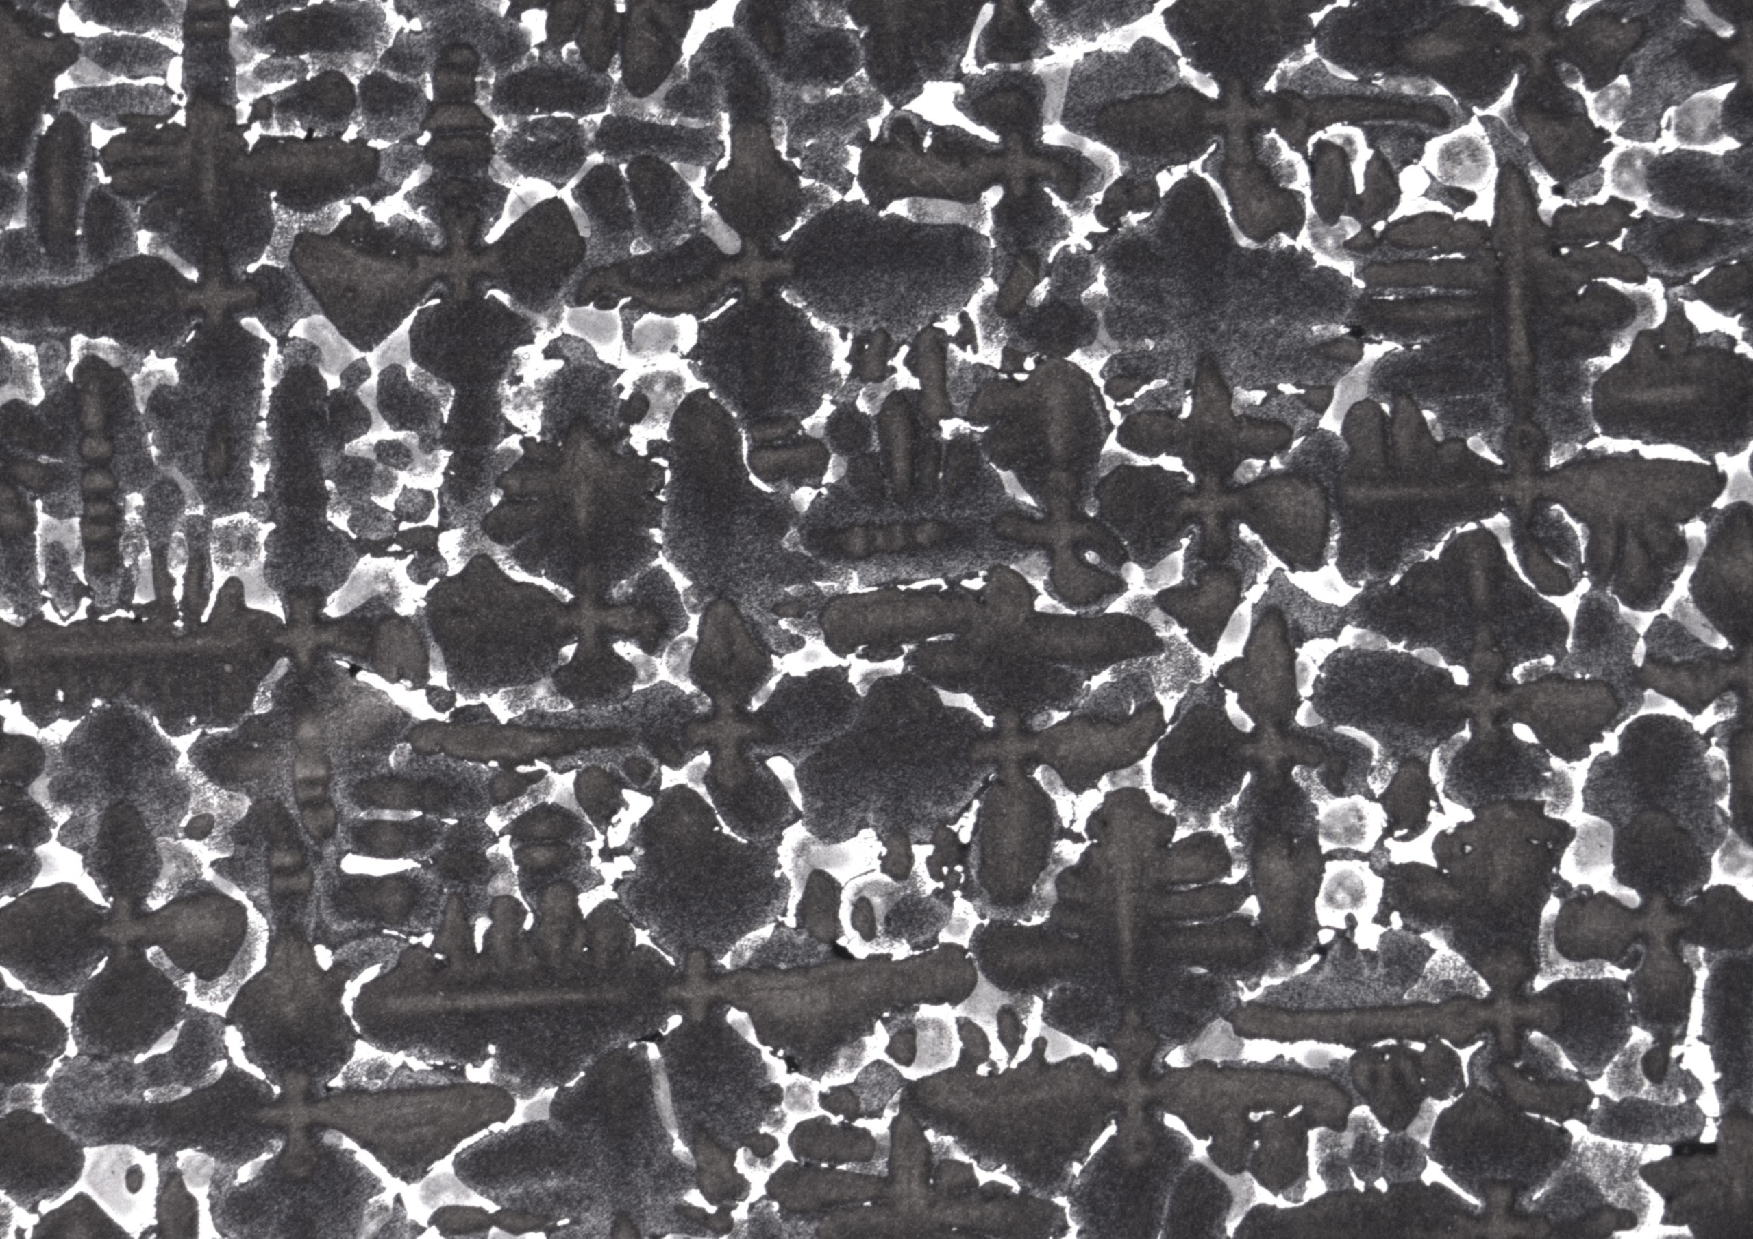
\includegraphics[width = 0.55\textwidth]{brut_dendrites.pdf}
    \caption{Observation des dendrites sur l'échantillon brut de fonderie
     au microsope optique, après traitement chimique à l'eau régale}
    \label{fig:brut_dendrites_optique}
\end{figure}

Nous obtenons un résultat clair : les dendrites (sombres, composées majoritairement
de phase $\gamma$) sont extrèmement développées et marquées en constrate de 
l'espace inter-dendritique (de couleur claire), qui a été attaqué par l'acide. 
Leur forme est dû au mécanisme de solidification successive de la pièce, 
lorsque le liquide se refroidit. Les dendrites croissent alors en partant 
de la base, et adoptent cette forme en sapin de Noël. Le matériau est donc inhomogène, 
ce qui nuit à ses qualités mécaniques. \\

%TODO : MEB

\subsection*{Echantillon remis en solution}

Regardons maintenant notre échantillon après la remise en solution. 
Ce traitement consiste à réchauffer la pièce à très haute température (\SI{1300}{\celsius}),
mais en-dessous du point de fusion de l'alliage : aucun liquide n'est donc formé. 

Ce traitement a pour but d'homogénéiser la composition de l'alliage. En effet, nous avons 
vu différentes zones se solidifient à différents moments, ce qui place une partie de l'alliage
hors équilibre (comme par exemple les agrégats eutectiques). Le chauffage intense va également 
permettre d'accèlérer la diffusion dans l'alliage, et donc faciliter le mouvement des atomes 
(notamment les plus lourds comme le rhénium). 

Observons donc notre échantillon ayant subit une étape de remise en solution au microscope optique.

\begin{figure}[H]
    \centering
    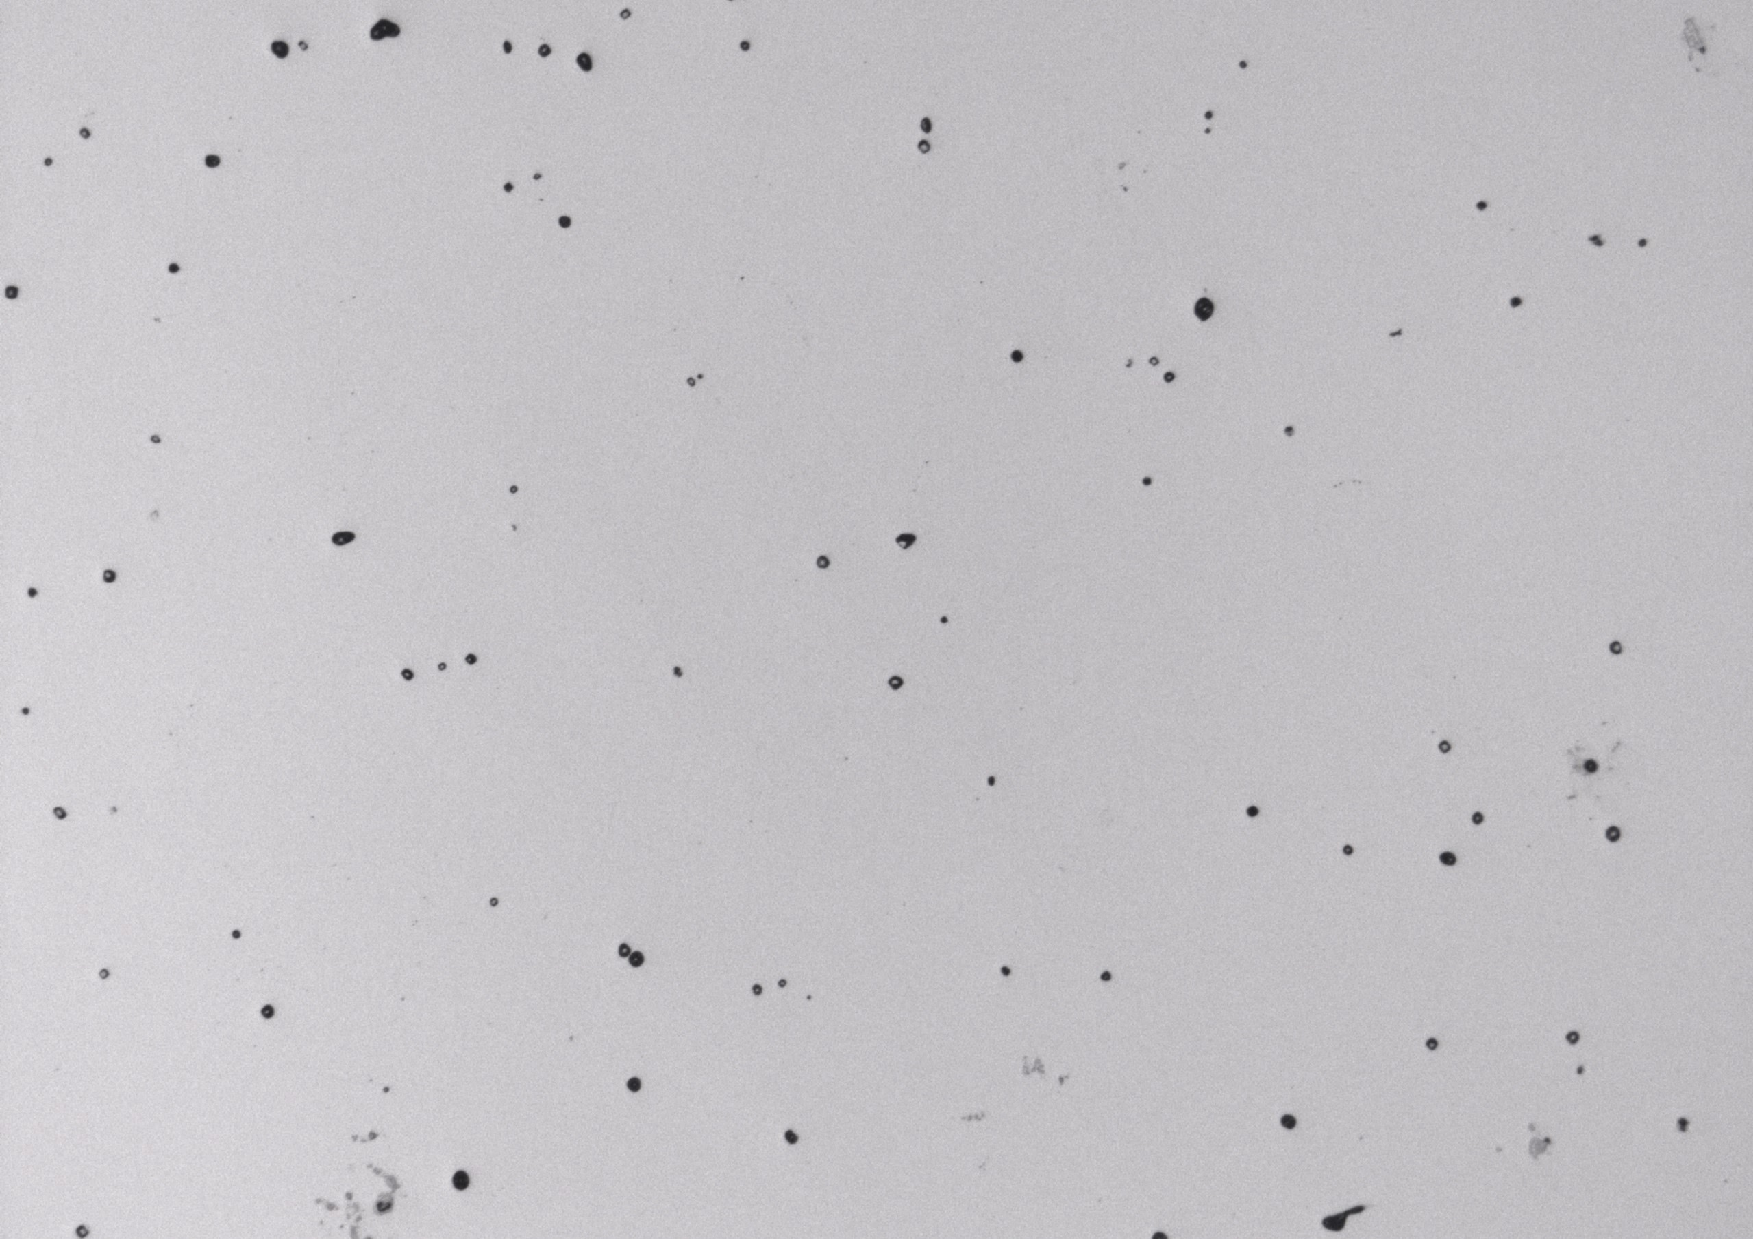
\includegraphics[width=0.55\textwidth]{images_optique/res.pdf}
    \caption{Echantillon après traitement de remise en solution}
    \label{fig:RES_optique}
\end{figure}

Nous voyons que les agrégats eutectiques, très visibles sur le brut, ont quasiment disparu.
Ils étaient en effet nettement hors équilibre et donc peu stables thermodynamiquement. 

Néanmoins, nous avons augmenté le nombre de pores. Cela est lié au fait que, la température 
augmentant, nous avons également augmenté la mobilité de tous les atomes et donc la possibilité
de former des pores en se refroidissant.\\

Il s'agit d'un effet indésirable du processus de remise en solution, d'autant plus que 
les deux traitements de revenu successifs ne parvienne pas à supprimer ces pores. 
Cependant, ce n'est pas un problème important car les bénéfices apportés par la diminution des 
agrégats eutectiques sont supérieurs, notamment en termes de résistance au fluage. \\

Nous obtenons les résultats suivants à l'aide d'ImageJ :

\begin{table}[H]
    \centering
    \caption{Proportion des différents défauts dans l'échantillon après remise en solution}
    \begin{tabular}{|c|c|}
        \hline
        \textbf{Type de défaut}  & \textbf{Proportion observée}  \\
        \hline
        Pore               & 0,525  \% \\
        Agrégat eutectique & 0,0041 \% \\
        \hline
    \end{tabular}
    \label{fig:proportion_defauts_RES}
\end{table}

Ces mesures corroborent nos observations visuelles.\\

Nous pouvons donc produire le graphique de comparaison suivant :


\begin{figure}[H]
    \centering
    % This file was created by tikzplotlib v0.9.8.
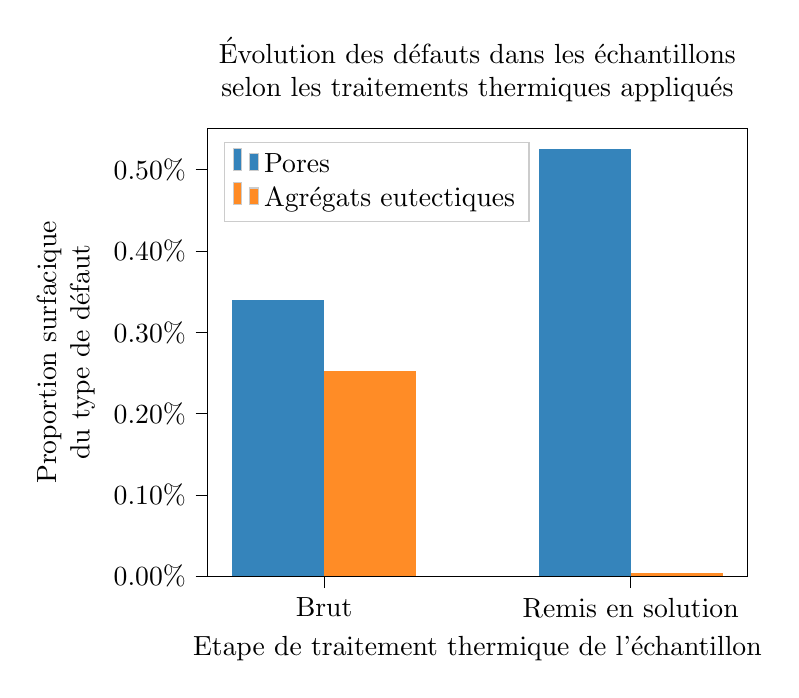
\begin{tikzpicture}

\definecolor{color0}{rgb}{0.12156862745098,0.466666666666667,0.705882352941177}
\definecolor{color1}{rgb}{1,0.498039215686275,0.0549019607843137}

\begin{axis}[
legend cell align={left},
legend style={
  fill opacity=0.8,
  draw opacity=1,
  text opacity=1,
  at={(0.03,0.97)},
  anchor=north west,
  draw=white!80!black
},
tick align=outside,
tick pos=left,
title={Évolution des défauts dans les échantillons\\selon les traitements thermiques appliqués},
x grid style={white!69.0196078431373!black},
xlabel={Etape de traitement thermique de l'échantillon},
title style = {align=center},
xmin=-0.23, xmax=1.53,
xtick style={color=black},
xtick={0.15,1.15},
xticklabels={Brut,Remis en solution},
y grid style={white!69.0196078431373!black},
ylabel={Proportion surfacique\\du type de défaut},
% ylabel style={text width=4cm},
ylabel style={align=center},
ymin=0, ymax=0.55125,
ytick style={color=black},
ytick={0,0.1,0.2,0.3,0.4,0.5,0.6},
yticklabels={0.00\%,0.10\%,0.20\%,0.30\%,0.40\%,0.50\%,0.60\%}
]
\draw[draw=none,fill=color0,fill opacity=0.9] (axis cs:-0.15,0) rectangle (axis cs:0.15,0.34);
\addlegendimage{ybar,ybar legend,draw=none,fill=color0,fill opacity=0.9};
\addlegendentry{Pores}

\draw[draw=none,fill=color0,fill opacity=0.9] (axis cs:0.85,0) rectangle (axis cs:1.15,0.525);
\draw[draw=none,fill=color1,fill opacity=0.9] (axis cs:0.15,0) rectangle (axis cs:0.45,0.252);
\addlegendimage{ybar,ybar legend,draw=none,fill=color1,fill opacity=0.9};
\addlegendentry{Agrégats eutectiques}

\draw[draw=none,fill=color1,fill opacity=0.9] (axis cs:1.15,0) rectangle (axis cs:1.45,0.0041);
\end{axis}

\end{tikzpicture}

    \caption{Évolution des défauts dans les échantillons selon les traitements thermiques appliqués\\}
    \label{fig:evolution_proportion_defauts_brut_RES}
\end{figure}

À nouveau, nous pouvons étudier notre échantillon après l'attaque chimique, 
afin de déterminer l'influence de la remise en solution sur les dendrites.\\

\begin{figure}[H]
    \centering
    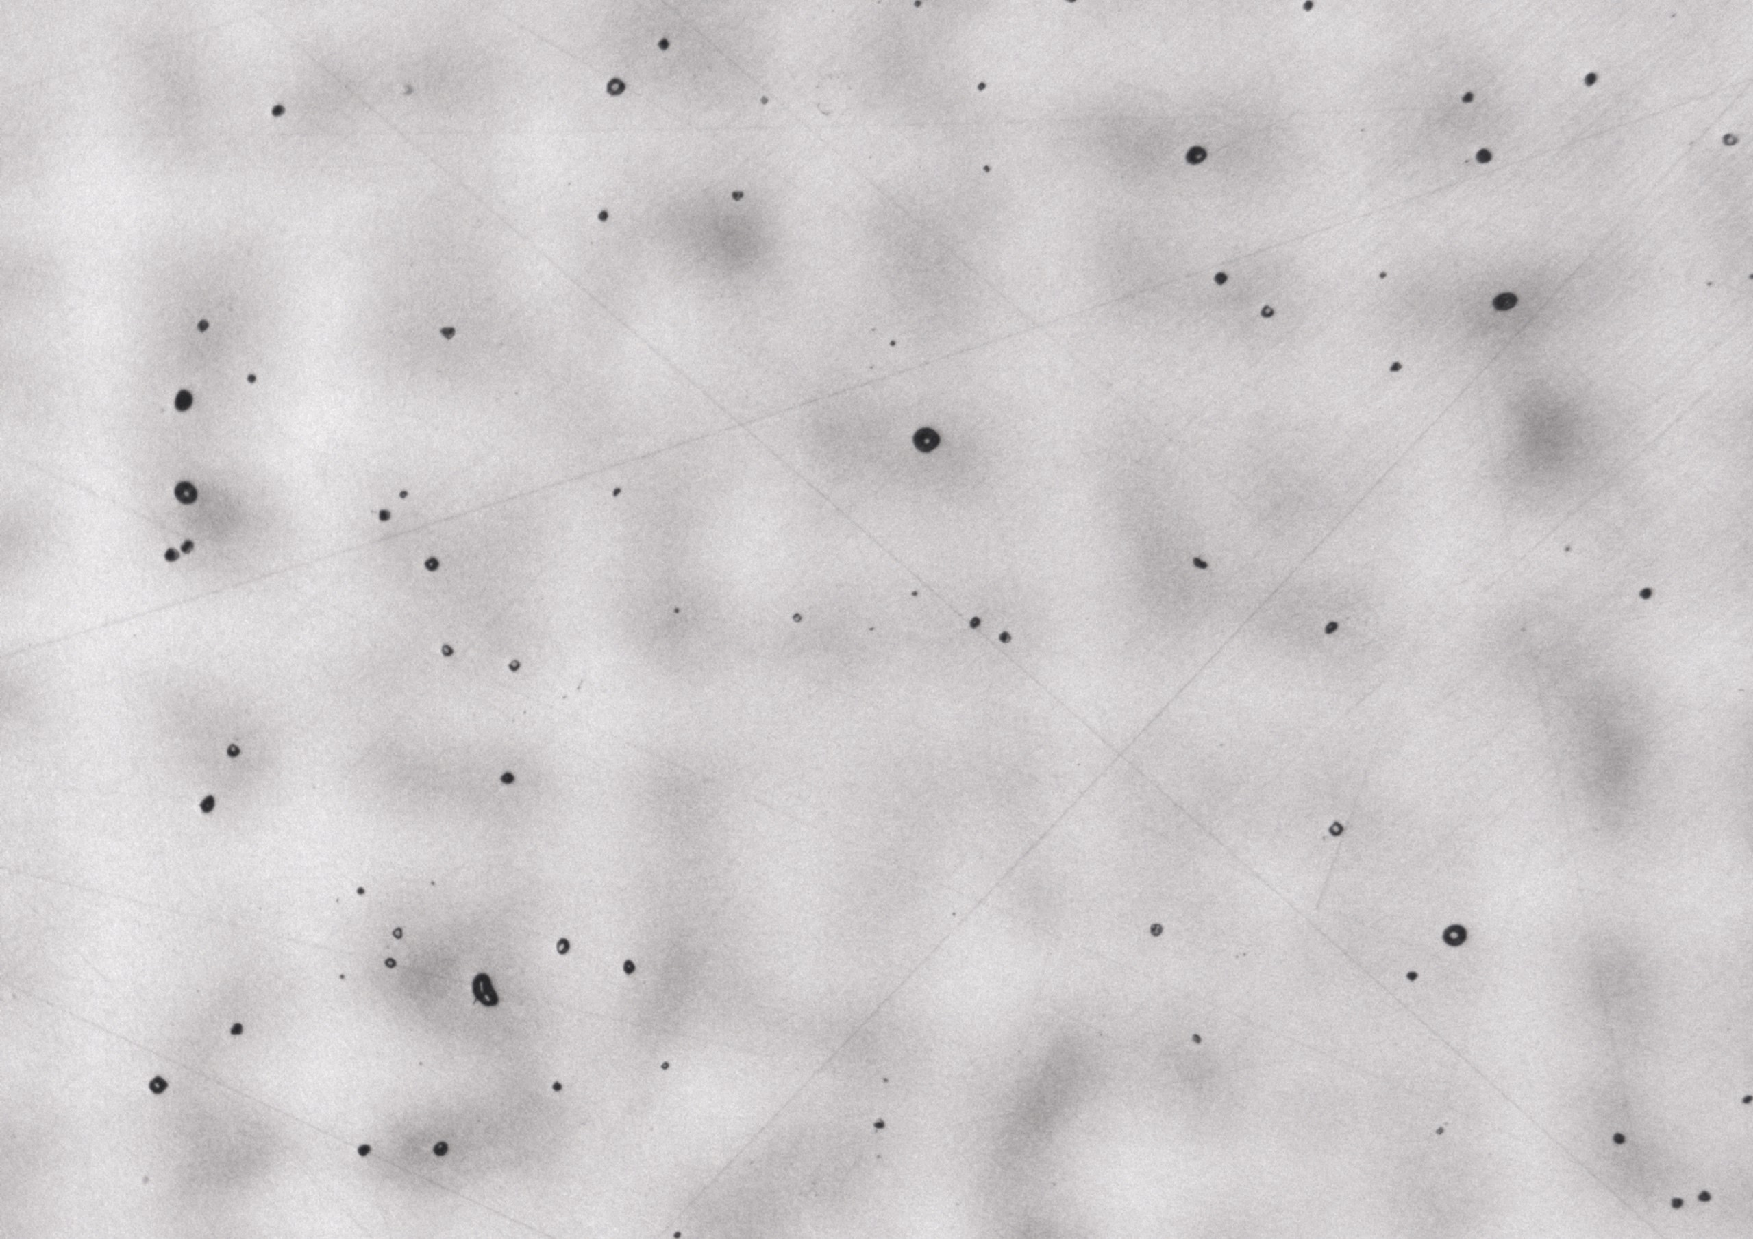
\includegraphics[width = 0.55\textwidth]{images_optique/res_dendrites.pdf}
    \caption{Observation des dendrites sur l'échantillon ayant subi une remise en solution
    au microsope optique, après traitement chimique à l'eau régale\\}
    \label{fig:res_dendrites_optique}
\end{figure}

Nous observons que, bien que la forme originelle des dendrites soit encore discernable, 
celle-ci est beaucoup plus atténuée. Nous avons donc réussi à homogénéiser nettement
la composition chimique de notre pièce, en enlevant d'une part les agrégats eutectiques, 
et d'autres part en "adoucissant" la frontière entre dendrites et espaces inter-dendritiques.


\subsection*{Conclusion sur les traitements thermiques}

La remise en solution permet donc d'améliorer nettement la qualité du matériau en
homogénéisant sa structure et en diminuant drastiquement le nombre d'agrégats
eutectiques, qui sont des endroits autours desquels la concentration n'est pas 
homogène, et dont la composition ne correspond pas au mélange $\gamma$/$\gamma'$
que l'on veut obtenir pour garantir les bonnes propriétés mécaniques de la pièce 
(résistance au fluage, résistance aux dislocations et déformations).



